\chapter{Selección y justificación del proveedor}

\section{Método de evaluación}

La decisión se tomó con una matriz multicriterio. Cada proveedor recibe una puntuación de 1 a 5, donde 1 indica ajuste bajo y 5 ajuste excelente. La nota ponderada se calcula como:

\[
S_j = \sum_{i=1}^{n} w_i r_{ij}, \qquad \sum_{i=1}^{n}w_i=1
\]

Aquí, $S_j$ es el resultado del proveedor $j$, $w_i$ el peso del criterio $i$ y $r_{ij}$ su calificación. Los pesos priorizan la adecuación de red y el beneficio académico porque el objetivo de la fase es aprender segmentación y demostrarla con bajo riesgo económico.

\begin{table}[H]
\centering
\caption{Criterios utilizados para seleccionar la nube}
\begin{tabularx}{\textwidth}{Y C{2.1cm} Y}
\toprule
\textbf{Criterio} & \textbf{Peso} & \textbf{Interpretación} \\
\midrule
Ajuste de red & 30\% & Claridad del modelo VPC, subredes, rutas y reglas de seguridad. \\
Beneficio académico & 25\% & Facilidad de construir una prueba corta con créditos o capa aplicable a la cuenta. \\
Documentación & 20\% & Cobertura oficial, ejemplos y capacidad de citar comportamiento exacto. \\
Infraestructura como código & 15\% & Madurez del proveedor Terraform y reproducibilidad. \\
Control de costo & 10\% & Visibilidad, etiquetas, presupuestos y facilidad de desmantelamiento. \\
\bottomrule
\end{tabularx}
\end{table}

\begin{figure}[H]
\centering
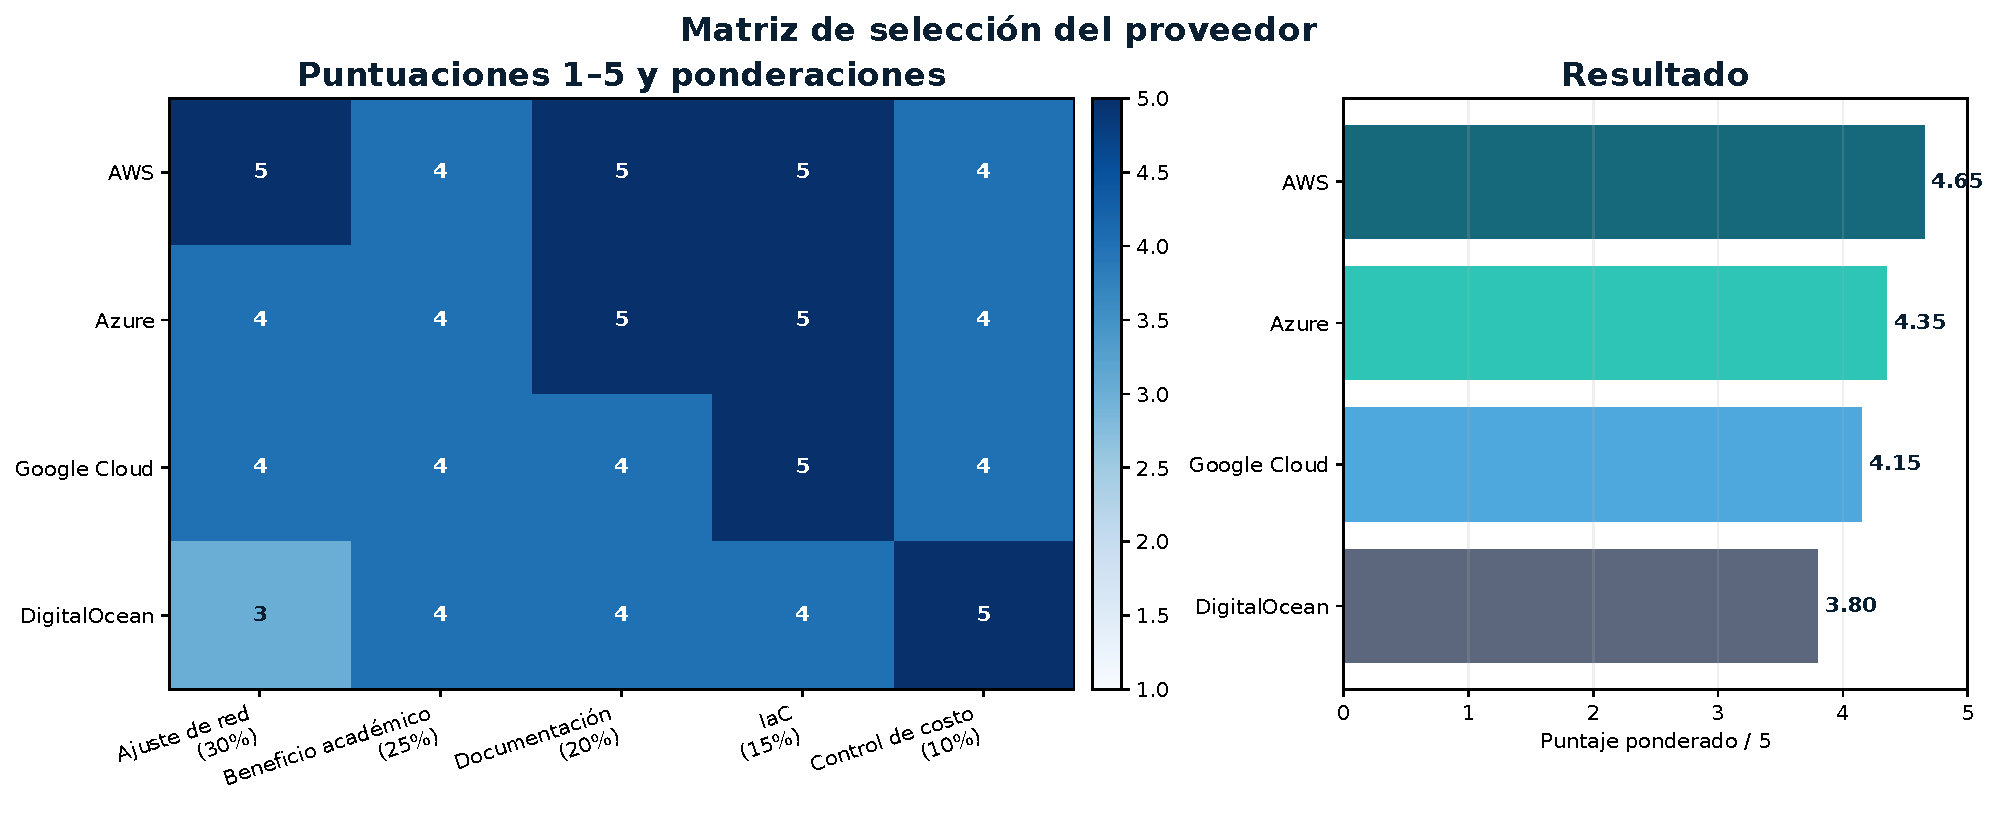
\includegraphics[width=\textwidth]{matriz-proveedores.pdf}
\caption{Matriz ponderada de selección del proveedor. Elaboración propia.}
\label{fig:providers}
\end{figure}

\section{Interpretación del resultado}

AWS obtiene 4.65/5, seguido por Azure con 4.35, Google Cloud con 4.15 y DigitalOcean con 3.80. La diferencia no implica que AWS sea universalmente superior; significa que ofrece el mejor ajuste para este prototipo y para los criterios definidos. Su documentación distingue con precisión subredes públicas y privadas: una subred es pública cuando su tabla contiene una ruta hacia un Internet Gateway, mientras una subred sin dicha ruta es privada \cite{aws-internet-gateway}.

Azure y Google Cloud ofrecen capacidades equivalentes y proveedores Terraform maduros, pero la nomenclatura de Amazon VPC se alinea de forma directa con los objetivos docentes del enunciado. DigitalOcean reduce complejidad operativa, pero esa misma simplificación ofrece menos elementos para demostrar rutas y controles de seguridad con el nivel de detalle buscado.

\section{Justificación técnica de AWS}

\subsection{Correspondencia entre conceptos académicos y recursos}

\begin{tabularx}{\textwidth}{p{4.2cm}Y}
\toprule
\textbf{Concepto de redes} & \textbf{Representación en el prototipo} \\
\midrule
Red empresarial privada & Amazon VPC con bloque RFC 1918 \code{10.10.0.0/24}. \\
Segmentación lógica & Cinco recursos \code{aws\_subnet} con CIDR no superpuestos. \\
Gateway & Internet Gateway adjunto a la VPC. \\
Enrutamiento & Tablas pública y privada asociadas explícitamente con las subredes. \\
Filtrado con estado & Grupos de seguridad para bastión y Ventas. \\
Host de prueba & Instancias EC2 con interfaces dentro de Ventas. \\
Documentación reproducible & Recursos declarativos y salidas de Terraform. \\
\bottomrule
\end{tabularx}

\subsection{Trazabilidad y automatización}

Terraform transforma la arquitectura en recursos declarativos revisables. El archivo de configuración permite detectar cambios, estandarizar etiquetas y recrear el entorno sin repetir pasos de consola. HashiCorp distribuye Terraform como un ejecutable multiplataforma y documenta el flujo de inicialización, planificación y aplicación \cite{terraform-install}. En el repositorio, cada componente se separa por propósito: proveedor, variables, red, seguridad, cómputo y salidas.

\subsection{Control del costo}

La elección se acompaña de límites concretos: el cómputo no se crea por defecto; no se incorpora NAT Gateway; sólo el bastión recibe una dirección pública; todas las instancias usan volúmenes pequeños y cifrados; y los recursos llevan la etiqueta \code{DeleteAfter=2026-10-19}. AWS recomienda rastrear recursos durante su ciclo de vida y retirar los elementos de prueba cuando dejan de ser necesarios \cite{aws-track-resources}. La automatización facilita cumplir esa práctica con \code{terraform destroy}.

\section{Decisión}

Se selecciona AWS para la Fase 1. La decisión está condicionada al alcance académico y debe reevaluarse si el proyecto evoluciona a producción, cambia el perfil de costos, requiere residencia de datos específica o necesita servicios administrados que alteren la comparación.
